%%%%%%%%%%%%%%%%%%%%%%%%%%%%%%%%%%%%%%%%%
% Wenneker Article
% LaTeX Template
% Version 2.0 (28/2/17)
%
% This template was downloaded from:
% http://www.LaTeXTemplates.com
%
% Authors:
% Vel (vel@LaTeXTemplates.com)
% Frits Wenneker
%
% License:
% CC BY-NC-SA 3.0 (http://creativecommons.org/licenses/by-nc-sa/3.0/)
%
%%%%%%%%%%%%%%%%%%%%%%%%%%%%%%%%%%%%%%%%%
%----------------------------------------------------------------------------------------
%	PACKAGES AND OTHER DOCUMENT CONFIGURATIONS
%----------------------------------------------------------------------------------------

\documentclass[10pt, a4paper, twocolumn]{article} % 10pt font size (11 and 12 also possible), A4 paper (letterpaper for US letter) and two column layout (remove for one column)

%%%%%%%%%%%%%%%%%%%%%%%%%%%%%%%%%%%%%%%%%
% Wenneker Article
% Structure Specification File
% Version 1.0 (28/2/17)
%
% This file originates from:
% http://www.LaTeXTemplates.com
%
% Authors:
% Frits Wenneker
% Vel (vel@LaTeXTemplates.com)
%
% License:
% CC BY-NC-SA 3.0 (http://creativecommons.org/licenses/by-nc-sa/3.0/)
%
%%%%%%%%%%%%%%%%%%%%%%%%%%%%%%%%%%%%%%%%%

%----------------------------------------------------------------------------------------
%	PACKAGES AND OTHER DOCUMENT CONFIGURATIONS
%----------------------------------------------------------------------------------------

\usepackage[english]{babel} % English language hyphenation

\usepackage{microtype} % Better typography

\usepackage{amsmath,amsfonts,amsthm} % Math packages for equations

\usepackage[svgnames]{xcolor} % Enabling colors by their 'svgnames'

\usepackage[hang, small, labelfont=bf, up, textfont=it]{caption} % Custom captions under/above tables and figures

\usepackage{booktabs} % Horizontal rules in tables

\usepackage{lastpage} % Used to determine the number of pages in the document (for "Page X of Total")

\usepackage{graphicx} % Required for adding images

\usepackage{enumitem} % Required for customising lists
\setlist{noitemsep} % Remove spacing between bullet/numbered list elements

\usepackage{sectsty} % Enables custom section titles
\allsectionsfont{\usefont{OT1}{phv}{b}{n}} % Change the font of all section commands (Helvetica)

%----------------------------------------------------------------------------------------
%	MARGINS AND SPACING
%----------------------------------------------------------------------------------------

\usepackage{geometry} % Required for adjusting page dimensions

\geometry{
	top=1cm, % Top margin
	bottom=1.5cm, % Bottom margin
	left=2cm, % Left margin
	right=2cm, % Right margin
	includehead, % Include space for a header
	includefoot, % Include space for a footer
	%showframe, % Uncomment to show how the type block is set on the page
}

\setlength{\columnsep}{7mm} % Column separation width

%----------------------------------------------------------------------------------------
%	FONTS
%----------------------------------------------------------------------------------------

\usepackage[T1]{fontenc} % Output font encoding for international characters
\usepackage[utf8]{inputenc} % Required for inputting international characters

\usepackage{XCharter} % Use the XCharter font

%----------------------------------------------------------------------------------------
%	HEADERS AND FOOTERS
%----------------------------------------------------------------------------------------

\usepackage{fancyhdr} % Needed to define custom headers/footers
\pagestyle{fancy} % Enables the custom headers/footers

\renewcommand{\headrulewidth}{0.0pt} % No header rule
\renewcommand{\footrulewidth}{0.4pt} % Thin footer rule

\renewcommand{\sectionmark}[1]{\markboth{#1}{}} % Removes the section number from the header when \leftmark is used

%\nouppercase\leftmark % Add this to one of the lines below if you want a section title in the header/footer

% Headers
\lhead{} % Left header
\chead{\textit{\thetitle}} % Center header - currently printing the article title
\rhead{} % Right header

% Footers
\lfoot{} % Left footer
\cfoot{} % Center footer
\rfoot{\footnotesize Page \thepage\ of \pageref{LastPage}} % Right footer, "Page 1 of 2"

\fancypagestyle{firstpage}{ % Page style for the first page with the title
	\fancyhf{}
	\renewcommand{\footrulewidth}{0pt} % Suppress footer rule
}

%----------------------------------------------------------------------------------------
%	TITLE SECTION
%----------------------------------------------------------------------------------------

\newcommand{\authorstyle}[1]{{\large\usefont{OT1}{phv}{b}{n}\color{DarkRed}#1}} % Authors style (Helvetica)

\newcommand{\institution}[1]{{\footnotesize\usefont{OT1}{phv}{m}{sl}\color{Black}#1}} % Institutions style (Helvetica)

\usepackage{titling} % Allows custom title configuration

\newcommand{\HorRule}{\color{DarkGoldenrod}\rule{\linewidth}{1pt}} % Defines the gold horizontal rule around the title

\pretitle{
	\vspace{-30pt} % Move the entire title section up
	\HorRule\vspace{10pt} % Horizontal rule before the title
	\fontsize{32}{36}\usefont{OT1}{phv}{b}{n}\selectfont % Helvetica
	\color{DarkRed} % Text colour for the title and author(s)
}

\posttitle{\par\vskip 15pt} % Whitespace under the title

\preauthor{} % Anything that will appear before \author is printed

\postauthor{ % Anything that will appear after \author is printed
	\vspace{10pt} % Space before the rule
	\par\HorRule % Horizontal rule after the title
	\vspace{20pt} % Space after the title section
}

%----------------------------------------------------------------------------------------
%	ABSTRACT
%----------------------------------------------------------------------------------------

\usepackage{lettrine} % Package to accentuate the first letter of the text (lettrine)
\usepackage{fix-cm}	% Fixes the height of the lettrine

\newcommand{\initial}[1]{ % Defines the command and style for the lettrine
	\lettrine[lines=3,findent=4pt,nindent=0pt]{% Lettrine takes up 3 lines, the text to the right of it is indented 4pt and further indenting of lines 2+ is stopped
		\color{DarkGoldenrod}% Lettrine colour
		{#1}% The letter
	}{}%
}

\usepackage{xstring} % Required for string manipulation

\newcommand{\lettrineabstract}[1]{
	\StrLeft{#1}{1}[\firstletter] % Capture the first letter of the abstract for the lettrine
	\initial{\firstletter}\textbf{\StrGobbleLeft{#1}{1}} % Print the abstract with the first letter as a lettrine and the rest in bold
}

%----------------------------------------------------------------------------------------
%	BIBLIOGRAPHY
%----------------------------------------------------------------------------------------

\usepackage[backend=bibtex,style=authoryear,natbib=true]{biblatex} % Use the bibtex backend with the authoryear citation style (which resembles APA)

\addbibresource{example.bib} % The filename of the bibliography

\usepackage[autostyle=true]{csquotes} % Required to generate language-dependent quotes in the bibliography
 % Specifies the document structure and loads requires packages

\usepackage{textalpha} % For unicode greek letters in normal text
\usepackage{amssymb, amsmath, amsthm, mathrsfs, enumitem, amsfonts, latexsym, bbm, stmaryrd, thmtools}
\usepackage{url}
\usepackage{graphicx}
\usepackage{xcolor}
\definecolor{svlinks}{rgb}{.0,0.3,0.6} %tmavě modrá
\usepackage[bookmarks,colorlinks=true,pdfhighlight=/O,linkcolor=svlinks,urlcolor=svlinks,citecolor=svlinks,
            pdftitle={PyVallex: A Processing System for Vallency Lexicon Data},
            pdfauthor={Anna Vernerová, Jonathan L. Verner},
            pdfsubject={},
            pdfkeywords={}
            ]{hyperref}
\usepackage{enumitem}
\usepackage{fouriernc}

\newcommand{\py}[1]{{\tt #1}}
\newcommand{\att}[1]{{\tt #1}}

%----------------------------------------------------------------------------------------
%	ARTICLE INFORMATION
%----------------------------------------------------------------------------------------

\title{PyVallex: A Processing System for Vallency Lexicon Data} % The article title

\author{
	\authorstyle{Anna Vernerov\'a\textsuperscript{1} and Jonathan L. Verner\textsuperscript{2,3}} % Authors
	\newline\newline % Space before institutions
	\textsuperscript{1}\institution{Institute of Formal and Applied Linguistics, Charles University, Prague}\\ % Institution 1
	\textsuperscript{2}\institution{Department of Logic, Charles University, Prague}\\ % Institution 2
	\textsuperscript{3}\institution{Institute of Formal and Applied Linguistics, Charles University, Prague} % Institution 3
}

% Example of a one line author/institution relationship
%\author{\newauthor{John Marston} \newinstitution{Universidad Nacional Autónoma de México, Mexico City, Mexico}}

\date{\today} % Add a date here if you would like one to appear underneath the title block, use \today for the current date, leave empty for no date

%----------------------------------------------------------------------------------------

\begin{document}

\maketitle % Print the title

\thispagestyle{firstpage} % Apply the page style for the first page (no headers and footers)

%----------------------------------------------------------------------------------------
%	ABSTRACT
%----------------------------------------------------------------------------------------

\lettrineabstract{We present PyVallex%AV:,
a Python-based system for display, editing and processing
of vallency lexicon data. The system consists of several components:
a parser for the specialized lexicon format used in several vallency lexicons,
a data-validation framework, a regular expression based search engine,
a map-reduce style framework for querying the lexicon data and a web-based interface integrating
complex search and some basic editing capabilities. Several of the components are provided
as a Python package allowing for programmatic access to the data.
}

%----------------------------------------------------------------------------------------
%	PREVIOUS WORK
%----------------------------------------------------------------------------------------
\section{Previous work}

%----------------------------------------------------------------------------------------
%	DESIGN OF THE SYSTEM
%----------------------------------------------------------------------------------------
\section{Motivation \& Design}
The main motivation for designing a system from scratch was that the mostly unstructured
nature of the previous system made it difficult to add new functionality and maintain the
system. The design of the system did not allow for easy integration into other tools which
was compounded by almost non-existing documentation. On the other hand, the older system
provided significant functionality which the new system needed to replicate.

AV: On the other hand, while many of the needed functionalities could be achieved through existing Dictionary Writing Systems (WDS; TODO: nejake odkazy),
it was a requirement that annotators could continue working as they were used to,
in other words, using the plaintext data format and Subversion revision system, for creating new entries as well as editing new ones.
It is expected that most annotators will learn to use selected features of PyVallex over time, especially the search/filtering functions, tabular output and editing of existing lexical units.
Moreover, the old system of custom-made scripts will be used used alongside PyVallex for some time, until all of its functionalities are fully implemented and tested.


The above considerations lead to the following design goals for the new system:

\paragraph{Modularity} To make adding new functionality easier, the system should be structured
into components, each with a well defined public interface (API). The components should only communicate
with each other through this API. This allows any new functionality to modify only the
relevant parts of the system and thus lowers the barrier for new contributors---a developer does
not need to have precise knowledge of the whole system to add/modify functionality to a single component.

\paragraph{Extendability} While the system should provide as much as possible of the functionality
already present in the older system, it should be designed from the start to be flexible and easily
extendible. In particular, it should have a well-defined data-model and provide an interface to allow
accessing the data from other programs (either through a library interface or, e.g., a REST API).

\paragraph{Maintainability} The design should aim to minimize the maintenance cost of the system.
In particular the system should be well documented, the components should be covered by an automated
test suite and the code style should be as uniform as possible and follow best practices.

Given the above goals, we have decided to implement the system in the \emph{Python 3} programming
language. Its advantage over \emph{Perl} (the language of the previous system) is that it provides
much better language support for structured programming. It is also becoming much more popular in
the NLP community, which makes it more likely that new contributors will be able to work with the
code. Although Python (as is the case also for Perl) is a weakly typed language, we have opted
to enforce the use of type hints via the mypy static type checker (\cite{tool:mypy}) run before every commit.
This makes the code effectively strongly-typed. In the interest of maintainability, we also enforce
a uniform coding style through the use of a commit-hook which runs autopep (\cite{tool:autopep8})
on the commited code.



%----------------------------------------------------------------------------------------
%	THE DATA LAYER
%----------------------------------------------------------------------------------------
\section{Data Layer}
A vallency lexicon consists of a collection of \emph{Lexemes}. A Lexeme represents a group of related
lexical units that share the same lemma or (as in the case of Vallex, NomVallex, and other lexicons) a group of derivationally related lemmas. Each lexical unit corresponds to a single meaning of these lemmas. Each lexical unit can be annotated
with a number linguistic properties,
e.g. AV: zpetne lomitko pred.mezeru
semantic (a gloss of the given meaning, level of abstraction,
indication of primary and metaphorical meanings),
syntactic (does the given LU enter syntactic structures such as passive, reflexive and reciprocal constructions? Which valency element of the given verb is referentially identical with the subject of the dependent infintive (a phenomenon called control)?
AV:... mozna moc podrobne a zase zahodit

The data layer definition is provided in the \py{vallex.data\_structures} module and consists of the
following classes \py{Lexicon} (representing a collection of \emph{lexemes}), \py{Lexeme} (representing
a single \emph{lexeme}), \py{LexicalUnit} (representing a \emph{lexical unit}), \py{Attrib} (representing a linguistically relevant property of a \emph{lexical unit}). The \py{Attrib} class also has several specializations: \py{Frame}
(representing the \emph{frame} annotation), \py{Lemma} (representing the \emph{lemma} annotation) and \py{SpecVal}
(representing the changes between a verb-noun derived pair). It is expected, that further sepcializations
will be defined to deal with particular properties.

Each of the above classes can store annotator provided textual comments (which can be used to explain
the reasoning behind a specific annotation, mark the data element as a work in progress, etc). They can also
store the original unparsed form (in the specialized annotator format
AV: original plaintext
) together with its location in the
source and they all provide a method to convert the data into a JSON representable structure.

%----------------------------------------------------------------------------------------
%	CORE COMPONENTS
%----------------------------------------------------------------------------------------
\section{Core components}
The core of the system consists of a \emph{parser module} which takes care of parsing the data and
constructing an in-memory representation of it---the data layer; a \emph{search module} which
provides query capabilities; a \emph{script module} which provides a framework for running data validation
and batch processing scripts; and an \emph{output module} which converts the in-memory representation into
various output formats. Each of these components is implemented in a python submodule of the main \py{vallex}
module and the components are mostly independent of each other.

%------------------------------------------------
\subsection{The parser}
The parse module takes care of parsing the specialized format (\autoref{fig:txt-fmt}) used by annotators when creating the lexicon data. The format (described in \cite{vallex}) is designed to be easily editable in any text editor and consise enough to facilitate manual creation.

\begin{figure}
\tiny
\begin{verbatim}
    : id: blu-v-brát-vzít-1
            ~ impf: brát (si) pf: vzít (si) iter: brávat (si)
            + ACT(1;obl) PAT(4;obl) ORIG(od+2;opt) LOC(;typ) DIR1(;typ) RCMP(za+4;typ)
                -synon: impf: přijímat; získávat pf: přijmout; získat
                -example: impf: brát si od někoho mzdu / peníze za práci;
                        pf: vzal si od něj peníze za práci;
                -note: mohli loni brát na odměnách.COMPL měsíčně 26 až 40 tisíc korun
                    volné si
                -recipr: impf: ACT-ORIG %berou si od sebe peníze%
                        pf: ACT-ORIG %nikdy si od sebe nevzali peníze%
\end{verbatim}
\caption{\label{fig:txt-fmt}Sample lexical unit in the textual format}
\end{figure}

The parser itself is split into a tokenizer function producing a stream of tokens and several
parse methods. The methods take care of constructing the \py{Lexeme}, \py{LexicalUnit}
and \py{Attrib} classes. It is designed in such a way that adding a specialized parser for
a newly introduced property is just a matter of writing a single function which is given
the body of the attribute and returns an instance of (a descendant) the \py{Attrib} class.
To integrate the function into the parser, it is enough to decorate it with a provided
Python decorator.

%------------------------------------------------
\subsection{Search}
The search module provides query capabilities to the system.

\paragraph{Queries} A query is a collection of conditions
and the result of the query is a set of lexical units each of which meets all
of the conditions of the query. Each condition consists of a \emph{selector} and a
\emph{pattern}. For each lexical unit the \emph{selector} is passed to a \py{match\_key\_values}
function which constructs a list of strings. A lexical unit satisfies the condition if at
least one of the strings matches the \emph{pattern}, which is a regular expression.
The \emph{selector} is a dot-separated list of strings. The standard implementation of the
\py{match\_key\_values} function interprets the first element of the selector as an attribute
name which it retrieves. It then passes the rest of the selector to the attribute's \py{match\_key\_values}
function to construct the list of strings to be matched against. The standard implementation
of the attribute's \py{match\_key\_values} method returns the attribute's textual representation
if the \emph{selector} is empty, its source form if the selector is 'src' and otherwise treats
the selector as a path through the attributes structure treated as a tre. It resolves the path and returns the
value present in the relevant node. For example a query consisting of the single condition
\begin{verbatim}
    example.pf=.*od.*
\end{verbatim}
would match the lexical unit shown in \autoref{fig:txt-fmt} whose \att{example} attribute
has the following structure
\begin{verbatim}
    {
        'impf': [ 'brát si od někoho mzdu /
                   peníze za práci'],
        'pf': ['vzal si od něj peníze za
                práci']
    }
\end{verbatim}
The \emph{selector} \att{example.pf} would retrieve the \att{example} attribute and from it
its \att{pf} node which contains the string \tt{vzal si od něj peníze za práci}. This string
incidentally matches the regular expression \tt{.*od.*}.

For discoverability purposes, each attribute has a method which returns a lists of all valid paths
inside its structure.

\paragraph{Executing queries}
The search module contains a \py{grep} method to execute queries. It additionally contains a \py{filter}
method which allows pruning each lexical unit from the result set so that it contains only the properties/attributes a user is interested in. Another method is provided to compute various histograms.
which allows




%------------------------------------------------
\subsection{Data Validation}
%------------------------------------------------
\subsection{Batch processing}
%------------------------------------------------
\subsection{Output}

%----------------------------------------------------------------------------------------
%	THE UI LAYER
%----------------------------------------------------------------------------------------

\section{The UI Layer}

\begin{figure}
    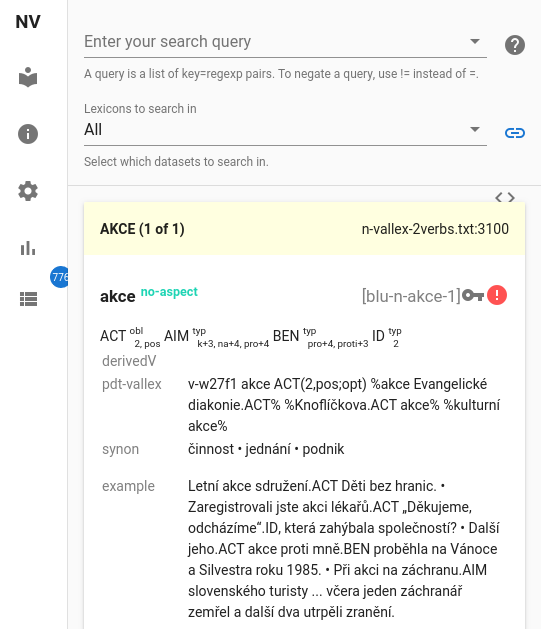
\includegraphics[width=\hsize]{images/ui-main.png}
    \caption{The main interface}
\end{figure}


%----------------------------------------------------------------------------------------
%	FUTURE WORK
%----------------------------------------------------------------------------------------


\section{Future work}



%----------------------------------------------------------------------------------------
%	BIBLIOGRAPHY
%----------------------------------------------------------------------------------------

\printbibliography[title={Bibliography}] % Print the bibliography, section title in curly brackets

%----------------------------------------------------------------------------------------

\end{document}
